\documentclass[en]{university}

\faculty{Department of Computer Engineering}
\course{Artificial Intelligence}
\subject{Mini Project 3 Theory Questions}
\professor{Dr. Rohban}
\student{Parsa Mohammadian}

\begin{document}

\setupdocument

\section{}

\subsection{}

We decide if a move violates game rules or not by using d-separation algroithm to find out 
if A and B are still independent. A valid move for each of the graphs is illustrated in 
figure \ref{fig:validmoves}.

\begin{figure}
    \centering
    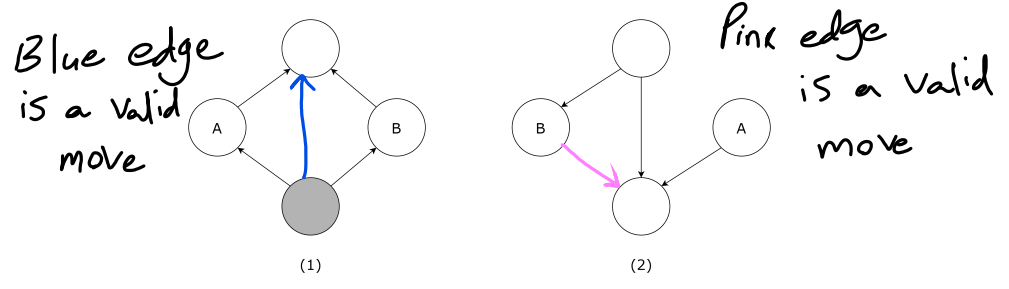
\includegraphics[width=0.8\textwidth]{assets/1-a.png}
    \caption{Valid Moves}
    \label{fig:validmoves}
\end{figure}

\subsection{}


\end{document}